% =====================================================================
% Transversal matroids in Lean 4 -- the tight-set architecture and the
% canonical obstruction.  First bead of the TotD strand drawn from the
% list "Theorems by Women Mathematicians".
% Authors: Carles Marín (Claude, Anthropic, as AI assistant).
% Style: clones the house line of godsil-gutman-lean.tex /
% neumann-separation-lean.tex: story-driven, one question per section,
% key formulas framed, Lean names in the tables, scope stated exactly.
% Build: pdflatex formalizing-transversal-matroids-in-lean4.tex (twice).
% Verified against the Lean source 2026-07-21:
%   lake build Theorems.TransversalObstruction  -> 1164 jobs, exit 0
%   #print axioms on the five headline theorems -> propext,
%   Classical.choice, Quot.sound only.  Toolchain leanprover/lean4:v4.32.0,
%   Mathlib revision 84fdd0bfb8e85237f54b9617cca79c6198d40a75 (2026-07-15),
%   local checkout E:\Mathlib\mathlib4.  Every priority/absence claim is
%   pinned to that revision and itemised in the Priority section.  The running example is
%   re-derived exhaustively by check_canonical_obstruction.sage before
%   every figure is drawn.
% =====================================================================
\documentclass[11pt]{article}
\usepackage[T1]{fontenc}
\usepackage{lmodern}
\usepackage{amsmath,amssymb,amsthm,booktabs,graphicx,hyperref,tabularx,array}
\usepackage{xurl}
\usepackage[table]{xcolor}
\definecolor{tmteal}{HTML}{1B6F8C}
\definecolor{tmband}{HTML}{DCE7EB}
\definecolor{tmamber}{HTML}{E08A1E}
\definecolor{tmplum}{HTML}{7B4B94}
\definecolor{tmgrey}{HTML}{B9C2CC}
\usepackage[margin=1in]{geometry}
\usepackage{microtype}
\usepackage{float}
\usepackage[most]{tcolorbox}
\usepackage{tikz}
\usetikzlibrary{arrows.meta,positioning,calc,fit,decorations.pathreplacing}
\setlength{\emergencystretch}{2em}
% Keep figures inline: a float should not claim a page it does not fill.
\renewcommand{\topfraction}{0.86}
\renewcommand{\bottomfraction}{0.72}
\renewcommand{\textfraction}{0.10}
\renewcommand{\floatpagefraction}{0.80}
\setlength{\intextsep}{9pt plus 2pt minus 2pt}
\setlength{\textfloatsep}{11pt plus 2pt minus 3pt}
\newtheorem{theorem}{Theorem}
\newtheorem{lemma}{Lemma}
\newtheorem{proposition}{Proposition}
\newtheorem{corollary}{Corollary}
\newcommand{\lean}[1]{\texttt{#1}}
\newcommand{\N}{\mathrm{N}}
\hypersetup{colorlinks=true,linkcolor=tmteal,citecolor=tmteal,urlcolor=tmteal}
\newtcbox{\keybox}{on line,boxrule=0.9pt,colframe=tmteal,colback=tmband!40,
  arc=3pt,left=8pt,right=8pt,top=5pt,bottom=5pt}
\newcommand{\keyeq}[1]{\begin{center}\keybox{$\displaystyle #1$}\end{center}}
\newtcolorbox{contribbox}[1]{colframe=tmamber,colback=tmamber!8,arc=3pt,boxrule=0.9pt,
  title=\textbf{#1},coltitle=white,colbacktitle=tmamber}
\newtcolorbox{recipebox}[1]{colframe=tmteal,colback=tmband!35,arc=3pt,boxrule=0.8pt,
  title=\textbf{#1},coltitle=white,colbacktitle=tmteal}

\title{\bf The Set That Says No\\[4pt]
  \large\normalfont Transversal matroids in Lean~4: a tight-set proof of augmentation,
  and the canonical obstruction it makes possible}
\author{Carles Mar\'in\thanks{Formalized with the assistance of an AI system (Claude,
Anthropic); the mathematics is classical, and every claim, scope statement, and limitation is
the author's responsibility. What is \emph{not} formalized is set out plainly in
Section~\ref{sec:boundary}, and the Lean kernel, not the assistant, is what certifies the
proofs.}\\[3pt]
  \normalsize Independent researcher\\
  \normalsize \texttt{karlesmarin@gmail.com}}
\date{July 2026}

\begin{document}
\maketitle

\begin{abstract}
Mathlib has Hall's marriage theorem. Mathlib has matroids. In the revision this work was
checked against (\lean{84fdd0bf}, 2026-07-15) nothing joins the two: every matroid in
\lean{Matroid/Constructions.lean} is trivial (\lean{emptyOn}, \lean{loopyOn}, \lean{freeOn},
\lean{uniqueBaseOn}), and none is built from combinatorial data. This
paper closes that gap for the classical bridge between them, the \emph{Transversal Matroid
Theorem} of Edmonds--Fulkerson and, independently, Mirsky--Perfect: for a finite family
$A=(A_0,\dots,A_{t-1})$ of finite sets, the partial transversals of $A$ are exactly the
independent sets of a matroid. I report a complete, \lean{sorry}-free Lean~4 formalization
over Mathlib of the finite-presentation form, packaged as \lean{transversalMatroid A} with
\lean{transversalMatroid\_indep} identifying its independent finite sets.

The contribution is not that Lean accepts the proof. It is the \emph{shape} of the proof. Rather
than certify an augmenting-path algorithm, the development runs Hall's obstruction method and
isolates one object in its own layer: a \emph{tight} set $R$, one whose compatible slots are
exactly saturated, $|\N(R)|=|R|$. A failed insertion produces a tight witness; tight sets are
closed under union; a union of witnesses forces $|J\setminus I|\le|I\setminus J|$, contradicting
$|I|<|J|$. Each step is a separate named lemma over Mathlib's finite matching interface, and
the separation pays a dividend the classical statement does not advertise. Since tight sets are
closed under intersection as well as union, they form a \emph{lattice}, so a partial transversal
$I$ carries a single largest tight subset $\lean{maxTight}\,A\,I$, and
\keyeq{\lean{insert}\;e\;I \text{ is a partial transversal} \iff \N(e)\not\subseteq \N(\lean{maxTight}\,A\,I),}
one canonical set deciding every insertion (\lean{insert\_iff\_not\_subset\_maxTight}). Put in
Mathlib's own vocabulary, that same set computes the matroid's closure operator on independent sets
(\lean{mem\_closure\_iff\_subset\_maxTight}): the library's apparatus applying to the constructed
object, rather than merely being said to apply. Six hundred and forty-five lines of Lean,
thirty-four theorems, no \lean{sorry}, \lean{admit} or
\lean{native\_decide}; \lean{\#print axioms} on all six headline theorems reports only
\lean{propext}, \lean{Classical.choice}, \lean{Quot.sound}. Section~\ref{sec:related} situates
the work against Hall, matching and matroid formalizations in Lean, Isabelle/HOL, Mizar and Coq,
and Section~\ref{sec:priority} states exactly which priority claims are made, what was searched to
support them, on what date, and what would refute them.
\end{abstract}

\medskip
\noindent\emph{What you will find here.} The paper follows the development in the order it was
built (Figure~\ref{fig:readermap}). Sections~\ref{sec:intro}--\ref{sec:related} say where the
formal state of the art stops and what exactly is added. Section~\ref{sec:q1} replaces the search
for a matching by a counting inequality, Section~\ref{sec:q2} turns the \emph{failure} of that
inequality into an object and proves augmentation from it, and Section~\ref{sec:q3} explains why
that route, split into three layers, is the contribution rather than a stylistic preference.
Section~\ref{sec:q4} packages the matroid; Section~\ref{sec:canonical} collects the dividend the
architecture pays. The load-bearing lemmas are in Section~\ref{sec:blocks}, the honest limits in
Section~\ref{sec:boundary}, the conclusion in Section~\ref{sec:conclusion}. If you read only two
things, read the contribution box at the end of Section~\ref{sec:intro} and
Theorem~\ref{thm:canonical}.

\begin{figure}[htbp]
\centering
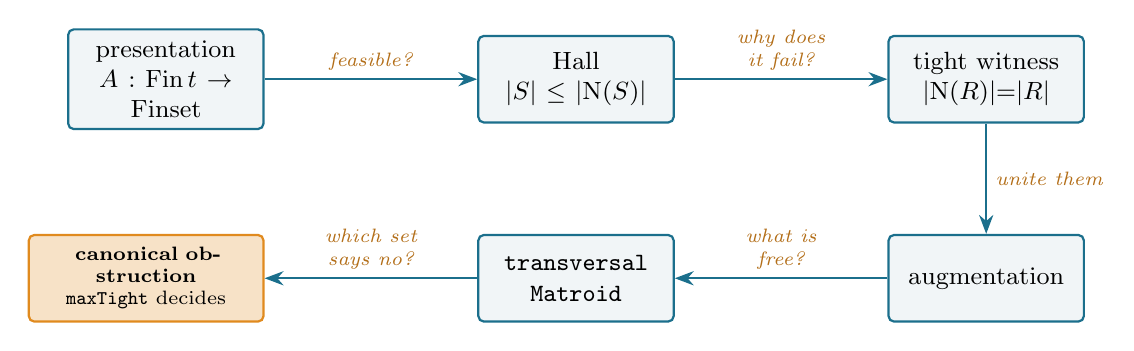
\begin{tikzpicture}[
  obj/.style={draw=tmteal,thick,rounded corners=2pt,fill=tmband!40,align=center,
    font=\small,inner sep=4pt,minimum height=11mm,text width=22mm},
  q/.style={font=\scriptsize\itshape,text=tmamber!80!black,align=center,fill=white,inner sep=1pt},
  arr/.style={-{Stealth[length=2.4mm]},thick,tmteal}]
  \node[obj] (pres) {presentation\\$A:\mathrm{Fin}\,t\to$ Finset};
  \node[obj,right=27mm of pres] (hall) {Hall\\$|S|\le|\N(S)|$};
  \node[obj,right=27mm of hall] (tight) {tight witness\\$|\N(R)|{=}|R|$};
  \node[obj,below=14mm of tight] (aug) {augmentation};
  \node[obj,left=27mm of aug] (mat) {\lean{transversal}\\\lean{Matroid}};
  \node[obj,left=27mm of mat,fill=tmamber!25,draw=tmamber,font=\scriptsize,text width=27mm] (can)
    {\textbf{canonical obstruction}\\\lean{maxTight} decides};
  \draw[arr] (pres) -- node[q,above=2pt] {feasible?} (hall);
  \draw[arr] (hall) -- node[q,above=2pt] {why does\\it fail?} (tight);
  \draw[arr] (tight) -- node[q,right=2pt,fill=none] {unite them} (aug);
  \draw[arr] (aug) -- node[q,above=2pt] {what is\\free?} (mat);
  \draw[arr] (mat) -- node[q,above=2pt] {which set\\says no?} (can);
\end{tikzpicture}
\caption{The reader's map. Every node is a block of \lean{sorry}-free Lean and every arrow is the
question its section answers. The chain runs left to right and back: from a finite presentation to
Hall's inequality, from a \emph{failure} of that inequality to a tight set, from many tight sets to
one, and from the matroid to the single canonical set that decides every insertion.}
\label{fig:readermap}
\end{figure}

% ---------------------------------------------------------------
\section{Two libraries that do not meet}\label{sec:intro}

Tasks must be assigned to distinct qualified agents. A task may have several compatible agents,
two tasks cannot share one agent, and the question is which collections of tasks can be served
\emph{simultaneously}. The compatibility relation is local and innocuous; the feasibility
condition is neither, because admitting one new task may force the reassignment of several old
ones. This is the terrain of systems of distinct representatives and of Hall's marriage
theorem~\cite{hall}.

Write the presenting family as
\[
  A=(A_0,\dots,A_{t-1}),\qquad A_i\subseteq\alpha,
\]
call $x$ \emph{compatible} with the index $i$ when $x\in A_i$, and call a finite set
$I\subseteq\alpha$ a \emph{partial transversal} when its elements can be assigned injectively to
compatible indices. The empty set is feasible; a subset of a feasible set is feasible, by
restricting the assignment. Neither observation reaches the fact that matters:

\begin{quote}
if $I$ and $J$ are partial transversals and $|I|<|J|$, then some $e\in J\setminus I$ makes
$I\cup\{e\}$ a partial transversal.
\end{quote}

That is the matroid exchange axiom, and it is not visible in the definition. Its history is worth
a paragraph, because this paper repeats it.

\emph{Two papers from 1935.} In the \emph{Journal of the London Mathematical Society}, Philip Hall
gave the exact condition for a family of sets to admit a system of distinct
representatives~\cite{hall}. In the \emph{American Journal of Mathematics}, Hassler Whitney
abstracted the properties of linear dependence and named the result a \emph{matroid}~\cite{whitney}.
They shared a year and little else: one asked when a set of choices can be made, the other
axiomatised what it means for choices to be independent, and neither refers to the other.

\emph{They stayed apart for a generation.} Whitney's paper drew a short burst of interest and then
matroid theory went quiet for over twenty years, until Tutte's papers of 1958--59 characterised the
regular and graphic matroids~\cite{farroxley}; Rado had meanwhile pursued the same ideas in the
1940s, proving the matroid generalisation of Hall's criterion~\cite{rado}. The revival came in the 1960s, and with it two
places where the two 1935 papers were finally read together. Jack Edmonds convened the first
conference on matroid theory at the National Bureau of Standards in 1965~\cite{oxleywelsh}; and at Sheffield, Leon
Mirsky, Hazel Perfect and John Pym were building transversal theory out of Hall's theorem and its
generalisations. Both groups arrived at the same bridge. The \emph{Journal of Research of the NBS}
carried Edmonds and Fulkerson's version in the conference year~\cite{edmondsfulkerson};
Mirsky and Perfect's, which also covers infinite families, appeared in 1967~\cite{mirskyperfect}.
Thirty years after 1935, the marriage theorem and the axioms of independence turned out to be
about one object.

\emph{Perfect kept going in that direction.} In 1968 she applied Menger's theorem to produce the
class of matroids now called \emph{gammoids}~\cite{perfect}---a class that contains the transversal
matroids~\cite{oxley,ingleton}, so that the object formalized in this paper is a special case of
one she introduced. Her doctorate followed the year after, in 1969, under the title \emph{Studies in
Transversal Theory with Particular Reference to Independence Structures and
Graphs}~\cite{perfectthesis}: the thesis came after the theorem. She was a Reader at Sheffield, wrote \emph{Independence Theory in
Combinatorics} with Victor Bryant in 1980~\cite{bryantperfect}, and the conjecture she made with
Mirsky in 1965 on which points of the unit disc are eigenvalues of $n\times n$ doubly stochastic
matrices~\cite{perfectmirsky}---proved by them for $n\le 3$, confirmed for $n=4$, refuted for
$n=5$---is open beyond that. Hers is the
name that puts this result on \emph{Theorem of the Day}'s list of theorems by women
mathematicians~\cite{totd}, from which the target was drawn; the attribution used throughout this
paper is the one that page prints.

\emph{Why it matters practically} is the greedy corollary. To say partial transversals form a
matroid is exactly to say that a cheapest maximal transversal can be selected greedily---cheapest
agents first, assignment settled afterwards---which is false for the naive matching search, where
a greedy prefix may have to be abandoned~\cite{totd}. The \emph{Theorem of the Day} page ends on
a caveat that this paper takes seriously and answers in Section~\ref{sec:canonical}: greediness
``leaves open the question of how we know our partial transversals are valid unless we find a
matching at the same time.''

\emph{Where formal libraries stand---which is to say, in 1935.} The situation this paper addresses
is the pre-1965 one, reproduced inside a proof assistant. Mathlib~\cite{mathlib}, the mathematical
library of Lean~4~\cite{lean4}, has Hall's marriage theorem, contributed by Gusakov,
{\sloppy Mehta and Miller~\cite{gusakov}, in the strong form we need: a finite matching interface
(\lean{hallMatchingsOn}) and the equivalence
\lean{Finset.all\_card\_le\_biUnion\_card\_iff\_existsInjective'}.\par} Mathlib also has a substantial
matroid development, due largely to Peter Nelson, with bases, circuits, closure, duality, minors
and rank. What it does not have is a bridge. Every matroid in
\lean{Mathlib/Combinatorics/Matroid/Constructions.lean} is trivial---\lean{emptyOn},
\lean{loopyOn}, \lean{freeOn}, \lean{uniqueBaseOn}---and none of them is built from combinatorial
data. Searching revision \lean{84fdd0bf} for \emph{transversal} returns the group-theoretic sense
(cosets, Schreier, Schur--Zassenhaus) and one prose mention inside the Hall module; there is no
transversal matroid. The two libraries sit beside each other and do not meet.

\begin{contribbox}{What this paper adds}
Existing formalizations of matching and of Hall's theorem do not, by themselves, yield a
transversal matroid: they certify \emph{that} a matching exists, and the matroid axiom needs a
reason \emph{why} an insertion fails. The contribution of this paper is threefold.
\begin{enumerate}\itemsep2pt
\item \textbf{The construction.} \lean{transversalMatroid A}, with its independent finite sets
identified exactly (\lean{transversalMatroid\_indep}), plugged into Mathlib's matroid API through
\lean{IndepMatroid.ofFinset}. To my knowledge, and against the searches dated and itemised in
Section~\ref{sec:priority}, it is the first matroid in Mathlib built from a combinatorial
presentation rather than by a trivial or dual construction---a statement about what I searched,
not a proof of absence.
\item \textbf{The proof architecture, which is the point.} Augmentation is proved by a
Hall-obstruction argument organized around \emph{tight} sets, split into three independent
layers---matching, tight-set, counting---each a separately named lemma. No augmenting-path
algorithm is formalized, and no monolithic tactic block appears. The tight-set layer is
library-shaped: it is about set families and Hall's inequality, not about matroids.
\item \textbf{The dividend that architecture pays.} Because the obstruction was isolated, one can
ask what tight sets do as a family. They are closed under intersection as well as union, hence
form a lattice; a partial transversal therefore has a \emph{maximum} tight subset
\lean{maxTight A I}, and a single containment test against it decides every insertion
(Theorem~\ref{thm:canonical}). That is not visible from the classical statement of the theorem, and
it is what the layered proof makes cheap.
\end{enumerate}
\end{contribbox}

% ---------------------------------------------------------------
\section{Related work}\label{sec:related}

The point of this section is orientation, not priority. Three literatures converge on the present
target---formal Hall theorems, formal matching theory, and formal matroid theory---and the
transversal matroid sits precisely where none of them ends up.

\paragraph{Hall's marriage theorem, formalized.} Hall's 1935 criterion~\cite{hall} is a standard
target for proof assistants. In Isabelle/HOL, Jiang and Nipkow contributed \emph{Hall's Marriage
Theorem} to the Archive of Formal Proofs in 2010~\cite{afphall}, with both the finite and the
countable-index versions. In Lean, Gusakov, Mehta and Miller formalized it in
Mathlib~\cite{gusakov}, in three interchangeable phrasings (indexed families of \lean{Finset}s, a
relation on finite types, and a \lean{Fintype} filter form), together with the compactness step of
Halpern that lifts the finite theorem to arbitrary index types. Neighbouring finite-set theorems
have been mechanized elsewhere---Dilworth's and Mirsky's theorems in Coq~\cite{coqdilworth}, and
Dilworth's again in the AFP (2025)---so the marriage theorem sits inside the settled part of the
formal combinatorics landscape rather than at its edge. \emph{What this gives and does not give.}
These developments certify the existence of a
system of distinct representatives under the Hall inequalities. They do not say what happens when
the inequalities fail, and the matroid axiom is entirely a statement about failure.

\paragraph{Matching theory, formalized.} Beyond the existence theorem, formal matching theory has
concentrated on algorithms and on the deeper structure theorems: Berge's augmenting-path
criterion, blossom-based maximum matching, and the algorithmic corner of combinatorial
optimization, chiefly in Isabelle/HOL. The most directly relevant entry is the ITP~2025
development \emph{A Formal Analysis of Algorithms for Matroids and Greedoids}~\cite{itp2025},
which includes executable bipartite maximum matching and verified greedy algorithms. This is the
piece of prior art closest to the present target and the reason no algorithmic claim is made here:
that literature already owns the algorithmic side. \emph{What this gives and does not give.} An
executable maximum-matching routine decides feasibility, and one can recover an obstruction by
inspecting a failed search. But the certificate is then an artifact of a particular algorithm run,
not an object with a theory; nothing in that route tells you that obstructions form a lattice.

\paragraph{Matroids, formalized.} Isabelle/HOL has Keinholz's AFP entry \emph{Matroids}
(2018)~\cite{afpmatroids}, developing independent sets, bases, circuits and rank, and the ITP~2025
matroid/greedoid algorithm work above. In Lean~4 the
largest matroid development is Peter Nelson's, which follows the infinite-matroid axioms and whose
core has been upstreamed into Mathlib; recent work in the same ecosystem includes a formalization
of the excluded-minor characterization of binary matroids~\cite{binarymatroids} and a verified
composition direction of Seymour's theorem for regular matroids~\cite{seymour}. The Lean matroid
area is active and structural. \emph{What this gives and does not give.} These libraries are rich
in what one can prove \emph{about} a matroid and poor in matroids to prove it about. Concretely,
in revision \lean{84fdd0bf} (2026-07-15) the constructions module offers only the empty, loopy,
free and unique-base matroids. Graphic matroids, linear matroids and transversal matroids---the
three classical families that make matroid theory a theory of examples---are, in that revision,
absent.

\paragraph{Transversal theory, formalized.} In searches carried out in July~2026 and itemised in
Section~\ref{sec:priority}, I located no formalization of the Transversal Matroid Theorem: not in
Lean/Mathlib (a text search of revision \lean{84fdd0bf} returns only the group-theoretic sense of
\emph{transversal}), not in the Isabelle AFP, not in Mizar, not in the Coq \lean{mathcomp}
ecosystem, and not in HOL~Light. This is
a negative search result and is recorded as such in Section~\ref{sec:boundary}: it is an audit
status, not a novelty claim, and the neighbouring AFP matroid/greedoid algorithm work is close
enough that any claim of first formalization of the surrounding \emph{area} would be false.

\paragraph{The gap, stated exactly.} Formal Hall theorems certify feasibility; formal matching
work certifies algorithms; formal matroid work certifies structure over an empty stock of
examples. The transversal matroid needs all three at once, and the join is not mechanical: the
matroid axiom is a statement about \emph{simultaneous} failure of many insertions, and no
existence theorem, however strong, delivers it. Supplying that join---with an obstruction object
factored out so that it can be reused and asked questions of---is what this paper does.

% ---------------------------------------------------------------
\section{Feasibility as a counting inequality}\label{sec:q1}

For an element $x$, the Lean development names its compatible indices
\lean{compatibleSlots A x : Finset (Fin t)}, and for a finite $S$ writes
\[
  \N(S)\;=\;\bigcup_{x\in S}\lean{compatibleSlots}\,A\,x
  \qquad(\lean{slotsOf}\ A\ S).
\]
\lean{IsPartialTransversal A I} is defined as the nonemptiness of Mathlib's
\lean{hallMatchingsOn (compatibleSlots A) I}: an injective function on the subtype of elements of
$I$, landing in the compatible slots. Putting the object in the library's own language, rather
than in a bespoke definition, is what makes the rest of the development short.

The first substantive result is the exact finite equivalence
\keyeq{I \text{ is a partial transversal} \iff |S|\le|\N(S)| \ \text{ for every } S\subseteq I .}
The forward direction restricts a matching to $S$ and injects $S$ into $\N(S)$; the reverse
delegates the construction of representatives to Mathlib's finite Hall theorem on the subtype of
elements of $I$. The asymmetry is deliberate proof engineering: one direction is a cardinal
injection we can do by hand, the other is exactly the library's job. In Lean the two halves are
\lean{partialTransversal\_hall} and \lean{hall\_partialTransversal}, paired as
\lean{partialTransversal\_iff\_hall}.

\begin{figure}[htbp]
\centering
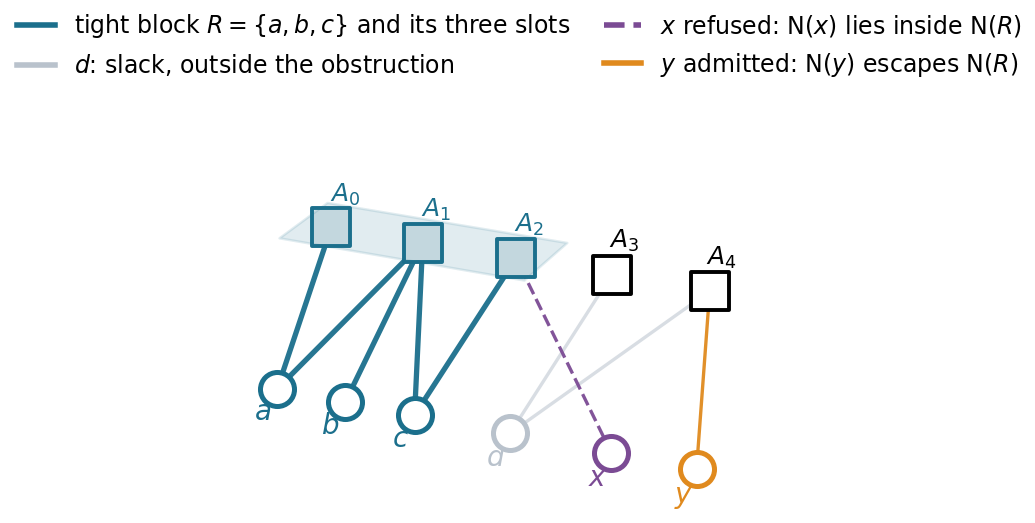
\includegraphics[width=0.86\linewidth]{figures/fig_presentation_3d.png}
\caption{The running example, drawn by \lean{generate\_obstruction\_figures.py} from the same data
that \lean{check\_canonical\_obstruction.sage} verifies. Five presenting sets over
$\{a,b,c,d,x,y\}$ give compatible slots $\N(a)=\{0,1\}$, $\N(b)=\{1\}$, $\N(c)=\{1,2\}$,
$\N(d)=\{3,4\}$, $\N(x)=\{2\}$, $\N(y)=\{4\}$. The set $I=\{a,b,c,d\}$ is a partial transversal
($a\!\mapsto\!0$, $b\!\mapsto\!1$, $c\!\mapsto\!2$, $d\!\mapsto\!3$). The shaded plane is the
saturated neighbourhood of the tight block $R=\{a,b,c\}$: three elements, three slots, nothing to
spare. It is the wall that refuses $x$ and lets $y$ through.}
\label{fig:presentation}
\end{figure}

Read on the example of Figure~\ref{fig:presentation}: for $I=\{a,b,c,d\}$ every subset has at
least as many slots as elements, so $I$ is feasible. For $\lean{insert}\,x\,I$ the subset
$\{a,b,c,x\}$ has four elements and only the three slots $\{0,1,2\}$; Hall fails at once. What
matters next is that this failure has a \emph{shape}. The question handed forward is: when every
attempted insertion fails, what do those failures share?

% ---------------------------------------------------------------
\section{Why a larger transversal must donate an element}\label{sec:q2}

Let $I,J$ be partial transversals with $|I|<|J|$, and suppose for contradiction that no
$e\in J\setminus I$ can be inserted into $I$.

For each such $e$, the Hall characterization gives $S\subseteq \lean{insert}\,e\,I$ with
$|\N(S)|<|S|$. Since $I$ itself satisfies Hall, $S$ must contain $e$ (otherwise $S$ would be a
violating subset of $I$); this is \lean{hall\_violation\_insert\_mem}. Remove $e$, call the
remainder $R$, and a short cardinality squeeze upgrades the strict inequality into four exact
facts:
\[
  R\subseteq I,\qquad e\notin R,\qquad |\N(R)|=|R|,\qquad \N(e)\subseteq \N(R).
\]

\begin{recipebox}{The tight witness (recipe)}
Call $R$ \textbf{tight} when it exactly saturates its compatible slots, $|\N(R)|=|R|$
(\lean{IsTight}): it has no slack at all. A tight $R\subseteq I$ with $\N(e)\subseteq\N(R)$ is a \emph{certificate that $e$ has
nowhere new to go}---every slot $e$ could use is already spoken for by elements of $R$, and $R$ has
no room to shuffle. In Lean the extraction is
\lean{exists\_tight\_witness\_of\_not\_insert}: a failed insertion is never an unexplained search
failure; it always hands back this object.
\end{recipebox}

On the running example with $I=\{a,b,c,d\}$, the attempt to add $x$ returns the tight witness
$R=\{a,b,c\}$: three elements filling the three slots $\{0,1,2\}$, and $\N(x)=\{2\}$ lies inside
them (Figure~\ref{fig:tight}).

\begin{figure}[htbp]
\centering
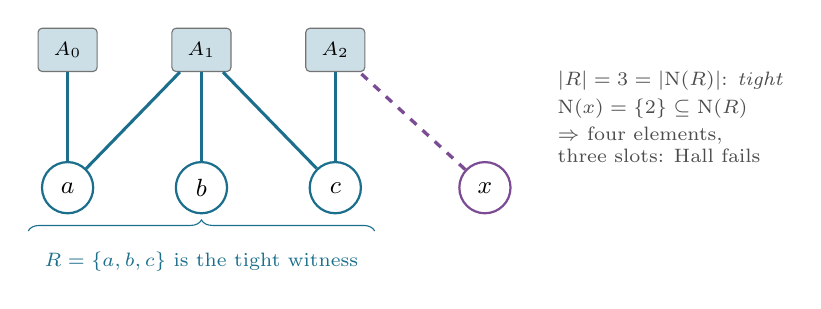
\begin{tikzpicture}[font=\small,
  el/.style={circle,draw=tmteal,thick,fill=white,inner sep=1.4pt,minimum size=6.5mm},
  sl/.style={rectangle,draw=black!55,rounded corners=1.5pt,inner sep=2pt,
    minimum width=7.5mm,minimum height=5.5mm,font=\scriptsize}]
  \foreach \i in {0,1,2} \node[sl,fill=tmteal!22] (s\i) at (1.7*\i,1.75) {$A_\i$};
  \foreach \x/\p in {a/0,b/1.7,c/3.4} \node[el] (\x) at (\p,0) {$\x$};
  \node[el,draw=tmplum] (x) at (5.3,0) {$x$};
  \draw[tmteal,line width=1.1pt] (a) -- (s0);
  \draw[tmteal,line width=1.1pt] (a) -- (s1);
  \draw[tmteal,line width=1.1pt] (b) -- (s1);
  \draw[tmteal,line width=1.1pt] (c) -- (s1);
  \draw[tmteal,line width=1.1pt] (c) -- (s2);
  \draw[tmplum,line width=1.2pt,dashed] (x) -- (s2);
  \node[align=left,font=\scriptsize,anchor=west,text=black!70] at (6.1,0.9)
    {$|R|=3=|\N(R)|$: \emph{tight}\\[2pt]
     $\N(x)=\{2\}\subseteq\N(R)$\\[2pt]
     $\Rightarrow$ four elements,\\three slots: Hall fails};
  \draw[decorate,decoration={brace,amplitude=4pt},tmteal] (-0.5,-0.55) -- (3.9,-0.55)
    node[midway,below=4pt,font=\scriptsize,text=tmteal]{$R=\{a,b,c\}$ is the tight witness};
\end{tikzpicture}
\caption{A failed insertion, explained rather than merely observed. The three shaded slots are
saturated by $\{a,b,c\}$, and every slot $x$ could occupy already lies among them. The certificate
is a set, not a trace of a failed search.}
\label{fig:tight}
\end{figure}

One tight set is local. Augmentation needs a \emph{single} obstruction covering all of
$J\setminus I$ at once, and the pivotal fact is that tightness survives union. If $R,S\subseteq I$
are tight then, because $\N(R\cup S)=\N(R)\cup\N(S)$ and $\N(R\cap S)\subseteq\N(R)\cap\N(S)$,
\keyeq{|\N(R\cup S)|+|\N(R\cap S)| \;\le\; |\N(R)|+|\N(S)| \;=\; |R|+|S| \;=\; |R\cup S|+|R\cap S| ,}
while Hall bounds each left-hand term from below by its right-hand partner. Both inequalities are
therefore forced to equalities, and $R\cup S$ is tight (\lean{tight\_union}); induction gives the
finite-family version \lean{tight\_biUnion}.

Now choose a tight witness $R_e$ for each $e\in J\setminus I$, set $U=\bigcup_e R_e$, and apply
Hall to $P=(J\setminus I)\cup(U\cap J)\subseteq J$. Its neighbourhood lies inside $\N(U)$, and $U$
is tight, so cardinal arithmetic yields $|J\setminus I|\le|I\setminus J|$
(\lean{card\_sdiff\_le\_of\_tight\_cover}). But for finite sets $|I|<|J|$ is equivalent to
$|I\setminus J|<|J\setminus I|$. Contradiction, and augmentation follows:
\begin{quote}\ttfamily\small\noindent
theorem partialTransversal\_augmentation\\
\hspace*{1em}(hI : IsPartialTransversal A I) (hJ : IsPartialTransversal A J)\\
\hspace*{1em}(hcard : I.card < J.card) :\\
\hspace*{1em}$\exists$ e $\in$ J \textbackslash\ I, IsPartialTransversal A (insert e I)
\end{quote}
This is a Hall/tight-set proof of augmentation. It does not implement maximum matching or
augmenting-path search: an existence theorem and a certified algorithm are different deliverables,
and only the first is claimed here.

% ---------------------------------------------------------------
\section{The three layers of the proof}\label{sec:q3}

The difficulty is not the empty set, not restriction, and not Hall's theorem, which Mathlib
already supplies. The genuine proof engineering is the route from \emph{several} failed insertions
to \emph{one} global contradiction. Written as a single argument it is a paragraph; written as a
single tactic block it is unreadable and unreusable. The development therefore separates it into
three layers, and this separation is the paper's central technical claim.

\begin{recipebox}{The three layers}
\textbf{Matching layer.} \lean{compatibleSlots}, \lean{IsPartialTransversal}, restriction, and
\lean{partialTransversal\_iff\_hall}: a stable interface between injective assignments and
cardinal inequalities. Everything above it speaks only of cardinalities.\\[3pt]
\textbf{Tight-set layer.} \lean{exists\_tight\_witness\_of\_not\_insert} turns a failure into an
object; \lean{tight\_union} and \lean{tight\_biUnion} give that object an algebra. This layer
mentions no matroid and no matching---only set families and Hall's inequality---which is exactly
why it is reusable, and why Section~\ref{sec:canonical} costs almost nothing.\\[3pt]
\textbf{Counting layer.} \lean{card\_sdiff\_le\_of\_tight\_cover} takes a finite family of tight
subsets covering the slots of $J\setminus I$ and returns the single inequality
$|J\setminus I|\le|I\setminus J|$. The augmentation theorem then merely chooses one witness per
element of the finite subtype $J\setminus I$ and invokes it.
\end{recipebox}

This is the formal analogue of drawing the obstruction before counting it. In Lean the details are
concrete: witnesses are indexed by a finite subtype and chosen with \lean{Exists.choose};
their union is a \lean{Finset.biUnion}; a neighbourhood is itself a \lean{biUnion}; the final
contradiction is \lean{Finset} union/intersection/difference arithmetic discharged by
\lean{omega}. None is deep in isolation. Keeping them in separately named lemmas is what stops a
short combinatorial paragraph from becoming one opaque proof, and it is what makes the tight-set
layer available to anyone who wants it for a different purpose.

The claim is worth stating without hedging: \emph{the novelty is not that Lean accepts the proof.
It is that the proof architecture isolates the tight-set obstruction into reusable lemmas.} That
is simultaneously a mathematical choice---obstruction method rather than augmenting paths---and a
proof-engineering one, and Section~\ref{sec:canonical} is the evidence that the choice was the
right one.

% ---------------------------------------------------------------
\section{Packaging the matroid}\label{sec:q4}

Mathlib's \lean{IndepMatroid.ofFinset} turns a finite-set independence predicate satisfying the
empty-set, hereditary and augmentation axioms into a finitary matroid. The development applies it
with ground set \lean{Set.univ} and predicate \lean{IsPartialTransversal A}:
\begin{quote}\ttfamily\small\noindent
noncomputable def transversalMatroid (A : Fin t $\to$ Finset $\alpha$) : Matroid $\alpha$
\end{quote}
The universal ground set is deliberate. An element of $\alpha$ occurring in no presenting set is
simply a \emph{loop}: no partial transversal contains it. The final theorem is therefore exact
without first restricting $\alpha$ to $\bigcup_i A_i$:
\begin{quote}\ttfamily\small\noindent
theorem transversalMatroid\_indep (A : Fin t $\to$ Finset $\alpha$) (I : Finset $\alpha$) :\\
\hspace*{1em}(transversalMatroid A).Indep (I : Set $\alpha$) $\leftrightarrow$ IsPartialTransversal A I
\end{quote}
This is the finite-presentation Transversal Matroid Theorem, as an object that downstream Mathlib
matroid results---rank, closure, bases, duality, minors---can consume directly;
Corollary~\ref{cor:closure} exercises the closure operator on it, so the claim is demonstrated
rather than asserted. The distinction
between an \emph{available} theorem and an \emph{implemented} application is kept: the
construction makes the interface available; it does not, here, implement a weighted greedy
optimizer, a rank oracle, or any complexity analysis.

% ---------------------------------------------------------------
\section{The obstruction is canonical}\label{sec:canonical}

Section~\ref{sec:q2} needed only that tight sets are closed under \emph{union}. Ask the tight-set
layer one more question---what about intersection?---and the same submodular squeeze answers it,
because the displayed chain of inequalities forces \emph{both} sides to equality at once. In Lean
this is a single lemma returning a conjunction, \lean{tight\_union\_and\_inter}; the intersection
half, \lean{tight\_inter}, is the half augmentation never uses.

\begin{proposition}[The tight sets are a lattice; \lean{tight\_union\_and\_inter}]\label{prop:lattice}
Let $I$ be a partial transversal and $R,S\subseteq I$ tight. Then $R\cup S$ and $R\cap S$ are
tight. Hence the tight subsets of $I$ form a sublattice of the Boolean lattice on $I$, containing
$\emptyset$.
\end{proposition}

That the equality cases of Hall's condition are closed under union and intersection is classical
matching theory---it is the submodularity of $\N$, the engine behind Ore's defect
formula~\cite{ore} and the Dulmage--Mendelsohn decomposition~\cite{dm}, and it is standard in
Lovász and Plummer~\cite{lovaszplummer}. Nothing new is claimed for the mathematics. What is new
is that the layered development gets it for the price of one extra conjunct, and that the
consequence below can then be stated at all.

Since the family is finite and closed under union, it has a maximum. The development defines
\[
  \lean{tightSubsets}\,A\,I=\{R\in\mathcal P(I) : R \text{ tight}\},\qquad
  \lean{maxTight}\,A\,I=\bigcup \lean{tightSubsets}\,A\,I ,
\]
and proves that this union is itself tight (\lean{maxTight\_isTight}, via \lean{tight\_biUnion})
and contains every tight subset (\lean{subset\_maxTight}). It is the \emph{maximum}, not merely a
maximal element.

\begin{figure}[htbp]
\centering
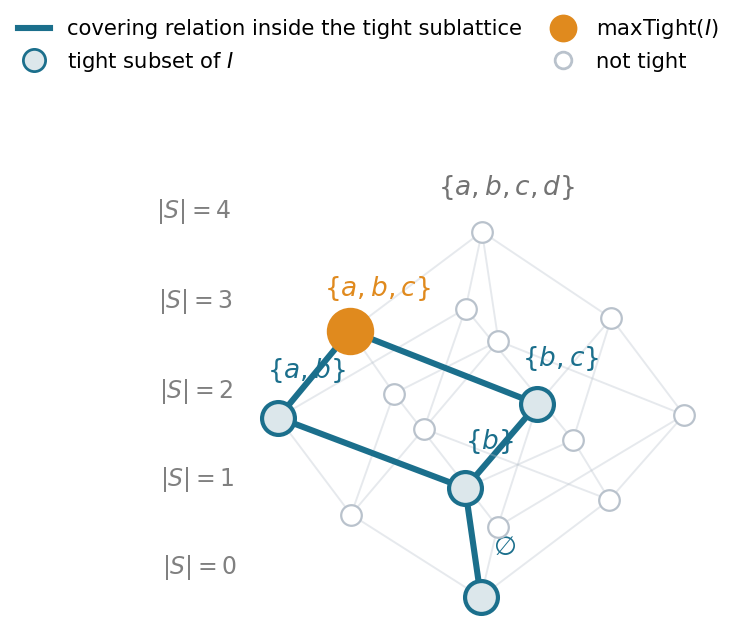
\includegraphics[width=0.62\linewidth]{figures/fig_lattice_3d.png}
\caption{The lattice of tight subsets of $I=\{a,b,c,d\}$, drawn inside the Boolean lattice on $I$
(height $=|S|$); $\lean{maxTight}(I)$ tops it, and $I$ itself is not tight. Only five of the sixteen subsets are tight, and they form a genuine lattice, not a
chain: $\{a,b\}\cap\{b,c\}=\{b\}$ and $\{a,b\}\cup\{b,c\}=\{a,b,c\}$ are both tight
(Proposition~\ref{prop:lattice}). The top, in amber, is $\lean{maxTight}(I)=\{a,b,c\}$---a
\emph{proper} subset of $I$, since $I$ itself has four elements and five slots. One containment
test against its neighbourhood decides every insertion.}
\label{fig:lattice}
\end{figure}

The reward is a decision statement. The existence lemma of Section~\ref{sec:q2} says a failed
insertion \emph{produces} a tight cover; its converse is elementary---if $R\subseteq I$ is tight,
$e\notin R$ and $\N(e)\subseteq\N(R)$, then $\lean{insert}\,e\,R$ has $|R|+1$ elements and only
$|R|$ slots, so Hall fails (\lean{not\_insert\_of\_tight\_cover}). Necessary and sufficient
together, and then monotonicity of $\N$ collapses the existential onto the maximum:

\begin{theorem}[One set decides every insertion; \lean{insert\_iff\_not\_subset\_maxTight}]
\label{thm:canonical}
Let $I$ be a partial transversal of $A$ and $e\notin I$. Then
\[
  \textnormal{\lean{insert}}\,e\,I \ \textnormal{is a partial transversal}
  \quad\Longleftrightarrow\quad
  \N(e)\ \not\subseteq\ \N\bigl(\textnormal{\lean{maxTight}}\,A\,I\bigr).
\]
\end{theorem}

\noindent The criterion is stated above in the development's own vocabulary. It can be said in
Mathlib's, and that is the form in which it becomes a statement about a matroid rather than about a
bespoke predicate:

\begin{corollary}[The obstruction computes the closure; \lean{mem\_closure\_iff\_subset\_maxTight}]
\label{cor:closure}
With $I$ and $e$ as above,
\[
  e\in(\textnormal{\lean{transversalMatroid}}\,A).\textnormal{\lean{closure}}\ I
  \quad\Longleftrightarrow\quad
  \N(e)\subseteq\N\bigl(\textnormal{\lean{maxTight}}\,A\,I\bigr).
\]
\end{corollary}

\noindent \lean{Matroid.closure} is Mathlib's own operator, carrying its own theory of flats,
spanning sets and rank; the corollary says that on independent sets that operator is decided by one
containment test against one canonical finite set---no search over subsets, no matching
recomputed. The proof is three lines: Mathlib's \lean{Indep.notMem\_closure\_iff\_of\_notMem} turns
membership in the closure into failure of an insertion, \lean{transversalMatroid\_indep} turns that
into a statement about partial transversals, and Theorem~\ref{thm:canonical} finishes. This is also
the promise of Section~\ref{sec:q4} discharged: the library's apparatus does apply to the
constructed object, and here it is applying.

This is the answer to the caveat \emph{Theorem of the Day} leaves open---how do we know our
partial transversals are valid without finding a matching at the same time? For a fixed $I$ we do
not need to: one tight set, computed once, answers every subsequent membership question by a
containment test. In the running example $\lean{maxTight}=\{a,b,c\}$ with $\N=\{0,1,2\}$, so
$\N(x)=\{2\}$ is inside and $x$ is refused, while $\N(y)=\{4\}$ is outside and $y$ is admitted
(Figure~\ref{fig:lattice}). An exhaustive cross-check over that presentation---all $56$ partial
transversals and all $180$ insertion decisions---agrees with the theorem in every case.

Two honest qualifications. First, \lean{maxTight} is defined by a filter over the powerset of $I$,
so the \emph{definition} is exponential; the theorem certifies the characterization, not an
efficient procedure, and computing the maximum tight set efficiently (it is a Dulmage--Mendelsohn
question) is left to the algorithmic literature. Second, as with Proposition~\ref{prop:lattice},
the mathematics is classical; the contribution is that it is formal, and that it fell out of the
architecture rather than requiring a new development.

% ---------------------------------------------------------------
\begin{figure}[htbp]
\centering
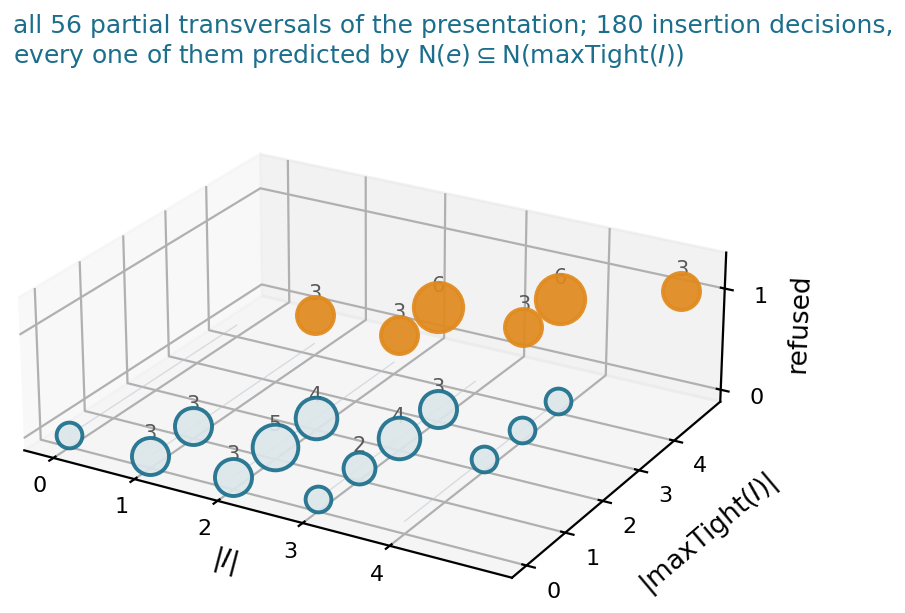
\includegraphics[width=0.72\linewidth]{figures/fig_decision_3d.png}
\caption{The criterion, exercised over the whole presentation rather than one example. Every
partial transversal $I$ of the running family is plotted at
$(|I|,\ |\lean{maxTight}(I)|,\ \#\text{refused})$, where a refusal means an element outside $I$
that cannot be inserted; marker area counts how many $I$ share a position. Amber marks the
positions where the canonical obstruction actually bites. All $56$ partial transversals and all
$180$ insertion decisions agree with Theorem~\ref{thm:canonical}; the plot is the exhaustive check
of \lean{check\_canonical\_obstruction.sage}, not a sample.}
\label{fig:decision}
\end{figure}

\begin{figure}[htbp]
\centering
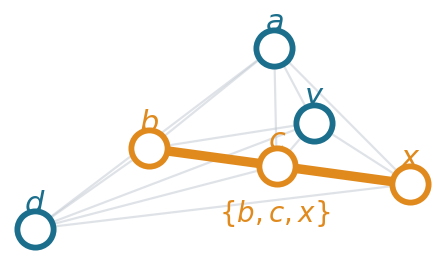
\includegraphics[width=0.74\linewidth]{figures/fig_circuit_3d.png}
\caption{The same presentation seen as the matroid it defines: rank~5 on six elements, so exactly
one circuit. Twelve of the thirteen rank-2 flats carry two points; one carries three, and the
drawing honours that by placing $b$, $c$ and $x$ on a line. That line \emph{is} the Hall violator,
$\N(\{b,c,x\})=\{A_1,A_2\}$---three points competing for two slots---and every refusal anywhere in
this presentation traces back to it. The circuit and the tight obstruction are the same
phenomenon read from opposite sides: a tight set is what remains of a circuit after one of its
elements is removed.}
\label{fig:circuit}
\end{figure}

\section{The building blocks}\label{sec:blocks}

Table~\ref{tab:results} gathers the load-bearing results; Table~\ref{tab:metrics} measures the
development. The dependency chain is short: the matching layer gives the Hall equivalence; the
Hall equivalence gives the tight witness; \lean{tight\_union\_and\_inter} gives the tight sets an
algebra; the counting layer turns a cover into one inequality; and the lattice gives the canonical
obstruction.

\begin{table}[H]
  \centering\footnotesize
  \arrayrulecolor{tmteal}
  \begin{tabular}{@{}llc@{}}
    \toprule
    \rowcolor{tmteal}
    \textcolor{white}{\textbf{Lean name}} & \textcolor{white}{\textbf{Statement}} & \textcolor{white}{\textbf{Status}} \\
    \midrule
    \multicolumn{3}{@{}l}{\emph{\lean{TransversalMatroid.lean}} --- the construction} \\
    \rowcolor{tmband}
    \lean{partialTransversal\_empty} & $\emptyset$ is a partial transversal & proved \\
    \lean{partialTransversal\_subset} & restriction of a matching (heredity) & proved \\
    \rowcolor{tmband}
    \lean{partialTransversal\_iff\_hall} & feasible $\iff$ $|S|\le|\N(S)|$ on all $S\subseteq I$ & proved \\
    \lean{hall\_violation\_insert\_mem} & a violating subset must contain $e$ & proved \\
    \rowcolor{tmband}
    \lean{exists\_tight\_witness\_of\_not\_insert} & failed insertion $\Rightarrow$ tight witness & proved \\
    \lean{tight\_union}, \lean{tight\_biUnion} & tightness survives finite union & proved \\
    \rowcolor{tmband}
    \lean{card\_sdiff\_le\_of\_tight\_cover} & $|J\setminus I|\le|I\setminus J|$ from a cover & proved \\
    \lean{partialTransversal\_augmentation} & the exchange axiom & proved \\
    \rowcolor{tmband}
    \lean{transversalMatroid\_indep} & \lean{Indep} $\iff$ partial transversal & proved \\
    \midrule
    \multicolumn{3}{@{}l}{\emph{\lean{TransversalObstruction.lean}} --- the canonical obstruction} \\
    \lean{tight\_union\_and\_inter} & tight sets form a lattice & proved \\
    \rowcolor{tmband}
    \lean{maxTight\_isTight} & the top of the lattice is tight & proved \\
    \lean{subset\_maxTight} & it is the maximum, not just maximal & proved \\
    \rowcolor{tmband}
    \lean{not\_insert\_of\_tight\_cover} & a tight cover blocks the insertion & proved \\
    \lean{not\_insert\_iff\_exists\_tight} & failure $\iff$ some tight cover & proved \\
    \rowcolor{tmband}
    \lean{insert\_iff\_not\_subset\_maxTight} & one set decides every insertion & proved \\
    \rowcolor{tmband}
    \lean{mem\_closure\_iff\_subset\_maxTight} & it computes \lean{Matroid.closure} & proved \\
    \bottomrule
  \end{tabular}
  \arrayrulecolor{black}
  \caption{The development, all \lean{sorry}-free, Lean~4 / Mathlib. \lean{\#print axioms} on
  \lean{partialTransversal\_augmentation}, \lean{transversalMatroid\_indep},
  \lean{tight\_union\_and\_inter}, \lean{maxTight\_isTight},
  \lean{insert\_iff\_not\_subset\_maxTight} and \lean{mem\_closure\_iff\_subset\_maxTight}
  reports only \lean{propext}, \lean{Classical.choice}, \lean{Quot.sound}.}
  \label{tab:results}
\end{table}

\begin{table}[H]
  \centering\footnotesize
  \arrayrulecolor{tmteal}
  \begin{tabularx}{0.96\linewidth}{@{}>{\raggedright\arraybackslash}p{0.36\linewidth}X@{}}
    \toprule
    \rowcolor{tmteal}
    \textcolor{white}{\textbf{Quantity}} & \textcolor{white}{\textbf{Value}} \\
    \midrule
    \rowcolor{tmband}
    Lines: construction $/$ obstruction & $400\,/\,245$ \\
    Theorems $+$ definitions & $15{+}4$ $/$ $19{+}5$ \\
    \rowcolor{tmband}
    Direct Mathlib imports & $3$: \lean{Combinatorics.Hall.Basic},
      \lean{Matroid.IndepAxioms}, \lean{Matroid.Closure} \\
    \lean{sorry} / \lean{admit} / \lean{native\_decide} & $0$ \\
    \rowcolor{tmband}
    Axioms beyond Lean's core & $0$: only \lean{propext}, \lean{Classical.choice},
      \lean{Quot.sound} \\
    Build & \lean{lake build}
      \lean{Theorems.TransversalObstruction} --- $1164$ jobs, exit~$0$ \\
    \rowcolor{tmband}
    Compile, warm Mathlib & ${\approx}\,4.7$\,s (obstruction module) \\
    Toolchain & Lean~4 \lean{v4.32.0}; Mathlib \lean{84fdd0bf} (2026-07-15) \\
    \rowcolor{tmband}
    Sage cross-check & $56$ partial transversals, $180$ insertion decisions \\
    \bottomrule
  \end{tabularx}
  \arrayrulecolor{black}
  \caption{The development measured. The footprint is deliberately light: two Mathlib imports, no
  heavy algebra, because the argument is elementary counting once the layers are separated. The
  Sage~\cite{sage} row is an executable cross-check of the running example, not evidence for the
  theorems; the Lean kernel is that evidence.}
  \label{tab:metrics}
\end{table}

% ---------------------------------------------------------------
\section{The boundary of the contribution}\label{sec:boundary}

\emph{What is proved.} The Transversal Matroid Theorem for finite presentations
\lean{A : Fin t $\to$ Finset $\alpha$}: partial transversals satisfy the three independent-set axioms and are
exactly the independent finite sets of \lean{transversalMatroid A}; plus the tight-set lattice, the
maximum tight subset, and the insertion criterion of Theorem~\ref{thm:canonical}. All
\lean{sorry}-free, with the axiom profile above.

\emph{Finite presentations only.} The family is finite and each $A_i$ is finite. The ambient type
$\alpha$ need not be finite, but the development characterizes the \emph{finite} independent sets
and uses Mathlib's finitary construction. The infinite version---the one Mirsky and Perfect also
proved~\cite{mirskyperfect}---is not covered.

\emph{No algorithmic claim.} The proof selects tight witnesses with classical choice. It proves
augmentation; it does not implement augmenting-path search, maximum matching, or any bound.
\lean{maxTight} is defined by a powerset filter and is not an efficient procedure.

\emph{The mathematics is classical.} Edmonds--Fulkerson and Mirsky--Perfect proved the theorem;
the tight-set method is standard transversal and matching theory~\cite{ore,dm,lovaszplummer,welsh,oxley}.
What is offered here is the formalization, its architecture, and the packaging of the obstruction
as a canonical object.

\emph{Authorship.} The formalization was carried out in close interaction with an AI assistant
(Claude, Anthropic): the choice of target, the proof architecture, the statements, and the scope
and novelty claims are mine; the assistant drafted and iterated much of the Lean under that
direction. This does not bear on validity---a proof is accepted only when the Lean kernel
type-checks it, which it does, with the axiom profile reported above---but it is stated plainly for
attribution.

\emph{Trust boundary.} The three reported axioms describe the theorems as checked by the current
Lean environment. They are not a claim to have eliminated the trusted Lean kernel, compiler, or
hardware.

% ---------------------------------------------------------------
\section{Priority: what was searched, when, and what would refute it}\label{sec:priority}

Claims of the form ``this had not been formalized'' decay. They are true of a moment, a set of
libraries and a set of queries, and every one of those changes. This section fixes all three so
that a reader in a later year can check the claim rather than trust it, and---if it has since
become false---can say exactly when it stopped being true.

{\sloppy\emph{What is claimed.} Two things, and nothing beyond them. (i) To my knowledge, the
matroid \lean{transversalMatroid} is the first in Mathlib constructed from a combinatorial
presentation rather than by a trivial or dual construction. (ii) To my knowledge, the Transversal
Matroid Theorem had not been formalized in an interactive theorem prover before this development.\par}
Both are claims about \emph{formalization}, never about the mathematics, which is
Edmonds--Fulkerson's and Mirsky--Perfect's and sixty years old.

\emph{What is not claimed.} No priority for any mathematical statement in this paper. No claim
that the surrounding area is unformalized---it is not: the AFP carries verified algorithms for
matroids and greedoids including bipartite maximum matching~\cite{itp2025}, and Mathlib carries a
substantial structural matroid theory. No claim about work I could not read, including unpublished
developments, private repositories, and formalizations filed under a different name.

\emph{Exactly what was searched, and when.} All of the following in July~2026.

\begin{itemize}\itemsep2pt
\item \textbf{Mathlib}, revision \lean{84fdd0bf} (2026-07-15), toolchain \lean{v4.32.0}: a
case-insensitive text search for \emph{transversal} over the whole of \lean{Mathlib/}, which
returns \lean{Combinatorics/Hall/Basic.lean} (prose only) and nine group-theoretic files
(\lean{GroupTheory/Complement}, \lean{CosetCover}, \lean{Schreier}, \lean{SchurZassenhaus},
\lean{Transfer}, and others), and no occurrence of \emph{transversal matroid}; plus a reading of
every declaration in \lean{Combinatorics/Matroid/Constructions.lean}, which defines exactly
\lean{emptyOn}, \lean{loopyOn}, \lean{freeOn} and \lean{uniqueBaseOn}.
\item \textbf{Isabelle/AFP}: the combinatorics topic index, and searches on \emph{transversal
matroid}, \emph{transversal}, \emph{matroid} and \emph{marriage}. Found: \emph{Matroids}
(Keinholz, 2018)~\cite{afpmatroids}, \emph{Hall's Marriage Theorem} (Jiang and Nipkow,
2010)~\cite{afphall}, and the ITP~2025 matroid/greedoid algorithm work~\cite{itp2025}. No
transversal-matroid entry located.
\item \textbf{Mizar, Coq/\lean{mathcomp}, HOL~Light}: searches on the same terms. Neighbouring
finite-set theorems were located in Coq~\cite{coqdilworth}; no transversal-matroid formalization
was located in any of the three. This is the weakest leg of the audit: it rests on public search
rather than on reading each library's index, and I would treat a pointer here as likely to
succeed before one aimed at Mathlib or the AFP.
\end{itemize}

\emph{What would refute it.} A single locator---library, entry name, file, date---for a
formalization of the Transversal Matroid Theorem, or for any Mathlib matroid built from
combinatorial data predating revision \lean{84fdd0bf}, refutes the corresponding claim outright.
Nothing else in this paper depends on either claim: the Lean development, the axiom profile, the
tight-set lattice and Theorem~\ref{thm:canonical} stand or fall on the kernel, not on priority.
I would be glad to be sent such a locator, and would record it.

% ---------------------------------------------------------------
\section{Conclusion}\label{sec:conclusion}

I formalized the Transversal Matroid Theorem for finite presentations in Lean~4 over Mathlib,
and packaged it as a matroid object, \lean{transversalMatroid A}, whose independent finite sets
are identified exactly by \lean{transversalMatroid\_indep}. To my knowledge---against the searches
dated and itemised in Section~\ref{sec:priority}, and subject to their stated limits---this is the
first matroid in Mathlib constructed from combinatorial data rather than from a trivial or dual
construction.

I proved augmentation---the one axiom the definition does not give away---by Hall's obstruction
method rather than by augmenting paths, and organized that proof into three independent layers:
a matching interface over Mathlib's finite Hall theorem, a tight-set layer with its own algebra,
and a counting layer that converts a cover of tight sets into a single cardinal contradiction.
Every step is a separately named, separately reusable lemma.

{\sloppy The resulting object integrates with Mathlib directly. It is produced through
\lean{IndepMatroid.ofFinset}, so the library's rank, closure, basis, duality and minor theory
applies to it without further work, and the ground set is taken universal, so that elements
outside every presenting set are loops and the characterization is exact. That integration is
exercised rather than asserted: Corollary~\ref{cor:closure} identifies Mathlib's own
\lean{Matroid.closure}, on independent sets, with a single containment test against
\lean{maxTight}.\par}

The architecture then paid for itself. Tight sets are closed under intersection as well as
union, hence form a lattice; every partial transversal has a maximum tight subset; and one
containment test against its neighbourhood decides every insertion
(Theorem~\ref{thm:canonical}). The obstruction is not an incident of a failed search but a
canonical invariant of the pair (presentation, independent set).

\emph{Future work}, in the order I would attempt it: extract an executable procedure returning
either an augmentation or the tight certificate, and connect it to the verified matching
algorithms of the Isabelle literature~\cite{itp2025}; carry Corollary~\ref{cor:closure} on to the
rank, where the value should be Ore's defect formula
$r(X)=\min_{S\subseteq X}\bigl(|X\setminus S|+|\N(S)|\bigr)$~\cite{ore}---verified exhaustively on
the running presentation by \lean{check\_canonical\_obstruction.sage}, and \emph{not} formalized,
which is exactly why it is future work rather than a result; lift the construction to
infinite indexed families, following Mirsky and Perfect and Mathlib's own compactness route for
Hall; and promote the tight-set layer to a standalone Mathlib contribution, since it is about
finite set systems and mentions no matroid at all.

% ---------------------------------------------------------------
\section{Reflections}\label{sec:reflections}

Formalizing a mid-1960s theorem is not, by itself, interesting. What the exercise taught is, and
these seven observations are the residue.

\paragraph{1. A theorem is not the same object as the reason it is true.}
The Transversal Matroid Theorem asserts that something \emph{can} always be done: a larger
transversal always donates. The proof, however, proceeds entirely by studying what \emph{cannot}
be done. Formalizing forced this asymmetry into the open, because a kernel will not accept ``one
sees that some element must work''; it demands a construction, and the only construction available
is of the obstacle. The negative object turned out to be the richer one---it has a lattice, a
maximum, and a decision procedure attached---while the positive statement has none of that. This
is worth stating as a working heuristic: when a theorem asserts that some choice exists, the
formalizable content usually lives in the classification of the reasons it might not.

\paragraph{2. Formal libraries are rich in theory and poor in examples.}
Mathlib can compute the dual, the minors, the rank and the closure of a matroid, and in revision
\lean{84fdd0bf} it had essentially no matroid to apply any of that to. The imbalance is structural
rather than accidental: theory is stated once and reused, while each family of examples---graphic,
linear, transversal---costs its own construction, and constructions get built last. The same
pattern is visible elsewhere in every large library. If one wants to be useful to a formal library
rather than merely present in it, building an example that its existing theory can chew on may be
worth more than another theorem about objects nobody has instantiated.

\paragraph{3. The layering was not tidiness; it was where the mathematics went.}
Splitting the proof into a matching layer, a tight-set layer and a counting layer was undertaken
for readability. It turned out to be the substantive act. Once the tight sets had their own layer,
asking whether they are closed under intersection was a natural question with a one-conjunct
answer, and Theorem~\ref{thm:canonical} followed. Had the augmentation proof been written as one
argument---as it is in the textbooks, and as it would have been in a first Lean attempt---the
lattice would have stayed invisible, because there would have been no object to ask the question
about. Proof engineering and mathematical discovery were, here, the same activity.

\paragraph{4. A certificate is worth more than a search.}
An augmenting-path algorithm answers ``can $e$ be inserted?'' by running, and answers again by
running again. The tight set answers once and is then reusable for every subsequent question about
the same $I$. \emph{Theorem of the Day}'s own caveat on this theorem---that greedy selection
``leaves open the question of how we know our partial transversals are valid unless we find a
matching at the same time''---is precisely a complaint about search, and the canonical obstruction
is the reply. That a refusal should come with a reason attached is a design principle that
generalizes well past matroids.

\paragraph{5. Classical does not mean available.}
Every mathematical ingredient here is decades old: Hall 1935, the theorem itself 1965--67, the
submodularity of the neighbourhood function older than either. Yet no proof assistant had the
statement, and the reason is not difficulty. It is that classical results are assembled from
prerequisites that libraries acquire in a different order than textbooks do, so the marginal cost
of a theorem in a library has little to do with its marginal cost on paper. This cuts both ways:
it explains why some celebrated theorems remain unformalized, and it means a modest classical
result can still be a genuine contribution to a library.

\paragraph{6. The right definition costs less than the clever proof.}
Defining \lean{IsPartialTransversal} as the nonemptiness of Mathlib's \lean{hallMatchingsOn}, and
not as a bespoke predicate, was the single decision that made the development short. It bought the
reverse Hall direction outright, and it made every later lemma a statement about cardinalities
rather than about functions. The corresponding temptation---to define a convenient predicate and
then prove it equivalent to the library's---would have added a translation layer to every proof.
Where a library already speaks about your object, it is almost always cheaper to speak its
dialect than to introduce your own.

\paragraph{7. What the assistant changed, and what it did not.}
This development was written in close interaction with an AI assistant, and it is worth being
precise about the effect. It compressed the mechanical distance between an idea and a checked
proof, so more architectural variants could be tried in an afternoon than would otherwise fit in a
week---and it was that cheap iteration, not any single insight, that surfaced the intersection
half of Proposition~\ref{prop:lattice}. What it did not change is the standard of truth. The
kernel accepted or refused, the axiom report is machine-generated, and the scope statements in
Section~\ref{sec:boundary} are claims a human is answerable for. A faster way to try things does
not lower the bar; if anything, it makes stating the bar explicitly more important.

% ---------------------------------------------------------------
\section{Open ends}\label{sec:questions}

Four questions the work raises but does not settle.

\begin{enumerate}\itemsep3pt
\item \emph{From witness to algorithm.} The tight witness already explains a refusal. Can the
existence proof be turned into a verified procedure returning either a larger transversal or a
checkable saturated-neighbourhood certificate---and does the maximum tight set, obtained from a
Dulmage--Mendelsohn decomposition, make that procedure polynomial with the certificate for free?
\item \emph{Which finiteness is really needed.} The proof uses finiteness in three separate
places: to choose witnesses, to take a finite union, and to do cardinal arithmetic. Which of the
three survives to infinite presentations, and is Mathlib's compactness argument for Hall enough to
carry the rest?
\item \emph{Does the tight-set layer belong in Mathlib?} \lean{tight\_union\_and\_inter} and
\lean{tight\_biUnion} say nothing about matroids. They are lemmas about a finite set system and
the equality case of Hall's condition. That is a Mathlib-shaped statement looking for a home.
\item \emph{One obstruction, three faces.} The lattice of tight sets is the same phenomenon as the
Dulmage--Mendelsohn decomposition of a bipartite graph and as the canonical maximal violator in
submodular optimization. Is there one Lean notion---a submodular function and its equality
lattice---that subsumes all three, with the transversal case an instance? That is the bead I would
most like to carry forward.
\end{enumerate}

% ---------------------------------------------------------------
\section*{Reproducing}

\begin{verbatim}
lake build Theorems.TransversalMatroid      # the construction
lake build Theorems.TransversalObstruction  # the canonical obstruction
lake env lean formalizations/transversal-matroid/lean/
              Theorems/AxiomReport.lean     # the trust report
python formalizations/transversal-matroid/sage/check_canonical_obstruction.sage
\end{verbatim}
{\sloppy Lean~4, toolchain \lean{leanprover/lean4:v4.32.0}, over Mathlib at revision
\lean{84fdd0bf} (2026-07-15):
\begin{center}
\url{https://github.com/leanprover-community/mathlib4}\\[2pt]
pinned at
\href{https://github.com/leanprover-community/mathlib4/commit/84fdd0bfb8e85237f54b9617cca79c6198d40a75}%
{\lean{84fdd0bfb8e85237f54b9617cca79c6198d40a75}}
\end{center}
The two Mathlib modules this development stands on, at that revision, are
\href{https://github.com/leanprover-community/mathlib4/blob/84fdd0bfb8e85237f54b9617cca79c6198d40a75/Mathlib/Combinatorics/Hall/Basic.lean}%
{\lean{Combinatorics/Hall/Basic.lean}} and
\href{https://github.com/leanprover-community/mathlib4/blob/84fdd0bfb8e85237f54b9617cca79c6198d40a75/Mathlib/Combinatorics/Matroid/IndepAxioms.lean}%
{\lean{Combinatorics/Matroid/IndepAxioms.lean}}; the constructions module whose contents
Section~\ref{sec:priority} reports is
\href{https://github.com/leanprover-community/mathlib4/blob/84fdd0bfb8e85237f54b9617cca79c6198d40a75/Mathlib/Combinatorics/Matroid/Constructions.lean}%
{\lean{Combinatorics/Matroid/Constructions.lean}}. Every absence claim in this paper is checkable
against those exact URLs, and remains checkable after Mathlib moves on. To reproduce elsewhere,
point \lean{lakefile.lean} at a compiled Mathlib with the same toolchain; the local path used here
is recorded in \lean{MATHLIB\_ENVIRONMENT.md}.\par}

{\sloppy The Lean sources, the generated axiom report, the exhaustive SageMath cross-check and the
deterministic figure generator are archived with the other formalizations of this
series~\cite{neumann,gglean,newtonlean} at
\url{https://github.com/karlesmarin/godsil-gutman-lean}. Both Lean files are \lean{sorry}-free, and
\lean{\#print axioms} on the six theorems listed under Table~\ref{tab:results} reports only
\lean{propext}, \lean{Classical.choice}, \lean{Quot.sound}. The source-level verification record is
\lean{VERIFICATION.md}; the running example of every figure is re-derived exhaustively---all $56$
partial transversals, all $180$ insertion decisions---by
\lean{check\_canonical\_obstruction.sage} before any figure is drawn.\par}

\begin{thebibliography}{99}\small
\bibitem{hall} P.~Hall, On representatives of subsets, \emph{J.~London Math.\ Soc.} \textbf{10}
(1935), 26--30. \url{https://doi.org/10.1112/jlms/s1-10.37.26}.
\bibitem{edmondsfulkerson} J.~Edmonds, D.~R.~Fulkerson, Transversals and matroid partition,
\emph{J.~Res.\ Nat.\ Bur.\ Standards Sect.~B} \textbf{69B} (1965), 147--153.
\bibitem{mirskyperfect} L.~Mirsky, H.~Perfect, Applications of the notion of independence to
problems of combinatorial analysis, \emph{J.~Combin.\ Theory} \textbf{2} (1967), 327--357.
\bibitem{perfect} H.~Perfect, Applications of Menger's graph theorem, \emph{J.~Math.\ Anal.\
Appl.} \textbf{22} (1968), 96--111. \url{https://doi.org/10.1016/0022-247X(68)90163-7}.
\bibitem{totd} R.~Whitty, The Transversal Matroid Theorem, \emph{Theorem of the Day},
\url{https://www.theoremoftheday.org/CombinatorialTheory/Transversal/TotDTransversal.pdf}
(attribution: ``proved in the mid-1960s by Jack Edmonds and Delbert Ray Fulkerson in the USA and,
independently (and also in an infinite version) by Leon Mirsky and Hazel Perfect at Sheffield
University in the UK'').
\bibitem{rado} R.~Rado, A theorem on independence relations, \emph{Quart.\ J.~Math.\ Oxford Ser.}
\textbf{13} (1942), 83--89 (Hall's criterion generalised to matroids).
\bibitem{perfectthesis} H.~Perfect, \emph{Studies in Transversal Theory with Particular Reference
to Independence Structures and Graphs}, Ph.D.\ thesis, University of London, 1969.
\bibitem{perfectmirsky} H.~Perfect, L.~Mirsky, Spectral properties of doubly-stochastic matrices,
\emph{Monatsh.\ Math.} \textbf{69} (1965), 35--57. \url{https://doi.org/10.1007/BF01313442} (the
source of the Perfect--Mirsky conjecture).
\bibitem{oxleywelsh} J.~Oxley, The contributions of Dominic Welsh to matroid theory,
\url{https://www.math.lsu.edu/~oxley/dominic.pdf} (on the Oxford and Sheffield schools, and on
Edmonds's 1965 National Bureau of Standards conference).
\bibitem{whitney} H.~Whitney, On the abstract properties of linear dependence, \emph{Amer.\ J.\
Math.} \textbf{57} (1935), 509--533 (the paper that names the matroid, published the same year as
Hall's).
\bibitem{farroxley} G.~Farr, J.~Oxley, The contributions of W.~T.~Tutte to matroid theory,
\url{https://www.math.lsu.edu/~oxley/Tutte_farrox5.pdf} (on the dormancy of matroid theory after
1935 and its revival with Tutte's papers of 1958--59).
\bibitem{bryantperfect} V.~Bryant, H.~Perfect, \emph{Independence Theory in Combinatorics: An
Introductory Account with Applications to Graphs and Transversals}, Chapman and Hall, 1980.
\bibitem{ore} O.~Ore, Graphs and matching theorems, \emph{Duke Math.\ J.} \textbf{22} (1955),
625--639 (the defect form of Hall's theorem).
\bibitem{dm} A.~L.~Dulmage, N.~S.~Mendelsohn, Coverings of bipartite graphs, \emph{Canad.\ J.\
Math.} \textbf{10} (1958), 517--534.
\bibitem{lovaszplummer} L.~Lov\'asz, M.~D.~Plummer, \emph{Matching Theory}, North-Holland, 1986.
\bibitem{welsh} D.~J.~A.~Welsh, \emph{Matroid Theory}, Academic Press, 1976.
\bibitem{oxley} J.~G.~Oxley, \emph{Matroid Theory}, 2nd ed., Oxford University Press, 2011.
\bibitem{ingleton} A.~W.~Ingleton, Transversal matroids and related structures, in \emph{Higher
Combinatorics}, NATO ASI Series~C \textbf{31}, Reidel, 1977, 117--131.
\bibitem{gusakov} A.~Gusakov, B.~Mehta, K.~A.~Miller, Formalizing Hall's marriage theorem in Lean,
2021. \url{https://arxiv.org/abs/2101.00127} (the Mathlib development used here:
\lean{Mathlib.Combinatorics.Hall.Basic}).
\bibitem{afphall} D.~Jiang, T.~Nipkow, Hall's Marriage Theorem, \emph{Archive of Formal Proofs}
(2010). \url{https://isa-afp.org/entries/Marriage.html}.
\bibitem{afpmatroids} J.~Keinholz, Matroids, \emph{Archive of Formal Proofs} (2018).
\url{https://isa-afp.org/entries/Matroids.html}.
\bibitem{coqdilworth} A.~Singh, R.~Natarajan, Fully mechanized proofs of Dilworth's theorem and
Mirsky's theorem, 2017. \url{https://arxiv.org/abs/1703.06133} (Coq; neighbouring finite-set
theorems).
\bibitem{itp2025} \emph{A Formal Analysis of Algorithms for Matroids and Greedoids},
\emph{Interactive Theorem Proving (ITP 2025)}, LIPIcs, Schloss Dagstuhl.
\url{https://drops.dagstuhl.de/entities/document/10.4230/LIPIcs.ITP.2025.2} (includes executable
bipartite maximum matching).
\bibitem{binarymatroids} \emph{Formalizing the Excluded Minor Characterization of Binary Matroids
in the Lean Theorem Prover}, University of Waterloo, 2023.
\url{https://uwspace.uwaterloo.ca/items/d35d17be-485d-4f60-8696-4dce7ae907bb}.
\bibitem{seymour} \emph{Composition Direction of Seymour's Theorem for Regular Matroids ---
Formally Verified}, 2025. \url{https://arxiv.org/abs/2509.20539}.
\bibitem{mathlib} The mathlib Community, The Lean mathematical library, in \emph{Certified
Programs and Proofs (CPP 2020)}, ACM, 2020, 367--381.
\url{https://doi.org/10.1145/3372885.3373824}. Repository:
\url{https://github.com/leanprover-community/mathlib4}; this work is checked against revision
\lean{84fdd0bfb8e85237f54b9617cca79c6198d40a75} (2026-07-15).
\bibitem{lean4} L.~de Moura, S.~Ullrich, The Lean~4 theorem prover and programming language, in
\emph{Automated Deduction (CADE~28)}, LNCS \textbf{12699}, Springer, 2021, 625--635.
\url{https://doi.org/10.1007/978-3-030-79876-5_37}. Repository:
\url{https://github.com/leanprover-community/lean4}.
\bibitem{sage} The Sage Developers, \emph{SageMath, the Sage Mathematics Software System}.
\url{https://www.sagemath.org}.
% --- this string of formalizations ---
\bibitem{neumann} C.~Mar\'in, \emph{When Separation Fails, a Canon Appears: one counting identity
behind separation, synchronization and symmetry-breaking in permutation groups, formalized in
Lean~4}, Zenodo, 2026. \texttt{doi:10.5281/zenodo.21419285} (the previous
\emph{Theorem of the Day} bead; same sourcing method, different cluster).
\bibitem{gglean} C.~Mar\'in, \emph{Random Signs into Matchings: A Godsil--Gutman Identity,
Formalized in Lean~4}, Zenodo, 2026. \texttt{doi:10.5281/zenodo.20517350} (matchings of a
bipartite graph, counted rather than chosen).
\bibitem{newtonlean} C.~Mar\'in, \emph{The Inward Bow of a Real-Rooted Polynomial: Newton's
Inequalities, Machine-Checked in Lean~4}, Zenodo, 2026. \texttt{doi:10.5281/zenodo.20693064}
(log-concavity, the classical ancestor of matroid log-concavity).
\end{thebibliography}

\end{document}
